% !TeX root = ../main.tex

\section{Random Forest}

Is a learning based approach for analyzing the feature space, with an ensemble of decision trees. A decision tree is a binary tree with a ``decision''\footnote{``Is this sample on the right side of a hyperplane?''} at every internal and the root node. It's a learning based approach, because good decision functions at the internal nodes are the result of training.

% \begin{figure}[H]
%   \centering
%   \includegraphics[width=0.2\textwidth]{decision_tree}
% \end{figure}

\paragraph{Training:} of a single tree in a forest of size $T$
\begin{enumerate}
  \item Select a number of splitting functions (\eg hyperplanes or conics, \dots)\footnote{simpler functions are typically preferred. Simplest function: ``axis aligned split''}
  \item Evaluate the information gain $I = H_{\text{before}} - H_{\text{after-l, weighted}} - H_{\text{after-r, weighted}}$ for each splitting function \footnote{where \(S_j\) is the data that flows into the node, \(S^L_j S^R_j\) is the data that flows to the left/right and \(H()\) denotes the entropy.}
  \[I = H(S_j) - \sum_{\mathclap{i \in \{L,R\}}}\ \ \frac{|S^i_j|}{|S_j|} H\left(S^i_j\right)\]
  \item Set the one with maximum information gain as the current node's decision function
  \item Recursively repeat for the child nodes, until max tree depth (or other stopping criteria\footnote{minimum number of samples for a split}) is reached
\end{enumerate}

If we have a trained decision tree, we can test it by evaluating the function at the root node.

\[h(\vec{x}, \vec{\vartheta}_j): \mathbb{R}^d \times \underset{\text{tree parameters}}{\mathcal{T}} \rightarrow \{0, 1\}\]

Depending on the result (0 or 1) we evaluate the test function at either the left successor or the right successor of the root node, and continue down the tree recursively until a terminal/leaf node is reached. This ``binary tree paradigm'' essentially performs a partitioning of the feature space, where the incoming samples are subdivided into two parts by each internal node.
The leaf node performs an application-specific action. For example, if the task is to perform classification, it assigns a label to the sample. Applications differ only in the computation of the information gain (objective function) and the "action" in the leaf node.

% compute the tree parameters \(\vartheta\), consisting of
\paragraph{Design parameters are:}
\begin{itemize}
  \item the tree height/depth\footnote{ trade-off: deeper trees tend to overfit, can be complemented with increased number of trees}
  \item the number of splitting functions at each internal node
  \item number of trees
\end{itemize}

\textit{Why an ensemble of trees?} Experience showed that it is complicated to train a single, highly accurate decision tree. The idea of random forests is therefore to train a large number of individually less accurate trees in a randomized fashion. Because of this randomization, each tree splits at a slightly different location, and thus the discontinuities are ``averaged out'' in the forest.

\paragraph{Randomization parameters:}
\begin{itemize}
  \item The candidate functions -- out of which the best one is chosen -- are randomly drawn
  \item if also linear projection of the data shall be drawn (\eg consider only dimensions \(\{d_{i_1}, d_{i_2}, \dots, d_{i_n}\}\)
  \item how the splitting parameters are sampled \footnote{a sparser sampling leads to more ``noise''/less optimal results (might be desired, e.g. prevents overfitting).}
  \item (how many candidate functions are drawn)
\end{itemize}

\subsection{Classification Forests}
Goal: Use the random forest model to train a classifier, which can be used to predict class labels.

\begin{figure}[H]
  \centering
  \includestandalone{classification-forest}
  %\includegraphics[width=0.3\textwidth]{space_partitioning}
  \caption{Possible space partitioning of one tree}
\end{figure}

The entropy in the classification case is defined as

\[H(S_j) = -\sum_{c \in C} p(c) \cdot \log(p(c))\]

where \(c\) denotes the class label, and \(p(c)\) the empirical distribution computed from \(S_j\).

% TODO: correct information gain
\[\Rightarrow I = H(S_j) - \sum_{\mathclap{i \in \{L,R\}}}\ \ \frac{|S^i_j|}{|S_j|} H\left(S^i_j\right)\]

\paragraph{Training:} basically the same as in the general case, but with the different objective function.
\begin{itemize}
    \item Possible stopping criterion if \eg 99\% of features in a node belong to one class
    \item Leaf nodes, report the relative frequencies of the class labels in that node (\eg 15\%: class 1, 85\% class 2)
\end{itemize}

The final classifier combines all trees by averaging the individual tree outputs. If a single discrete label is required, decide for the class with maximum probability.


\subsection{Regression Forests}
Goal: Use the random forest model to predict a \underline{continuous} label \(p(y|\vec{x})\).

(Remark: choice of the model complexity is related to the bias/variance trade off)

``Leaf prediction model'': a base function that is fitted to the samples. The leaf prediction model could be constant (maximize the bias), linear, polynomial, \dots

To faithfully represent all of the data with a single function, it would certainly make sense to use a polynomial model, or something even more complex. However, the random idea implies to subdivide/partition the space, and to fit simpler models to the individual partitions.

\begin{figure}[H]
	\centering
  \includegraphics[height=4cm]{rf_regression}
	\caption{ (Linear) regression split}
\end{figure}

The decision criterion for the splitting function works analogously to the classification case. The only difference is that we need to define the entropy on continuous values:

\[H(S_j) = -\frac{1}{|S_j|} \cdot \sum_{\vec{x} \in S_j} \int_y p(y|\vec{x}) \cdot \log(y|\vec{x})\dif y\]

where \(p(y|\vec{x})\) can, e.g. be chosen as a Gaussian distribution \(p(y|\vec{x}) = \mathcal{N}(y; \overline{y}(\vec{x}), \sigma_y^2(\vec{x}))\), where \(\overline{y}(\vec{x})\) is a linear function and \(\sigma_y(\vec{x})\) is the conditional variance computed from a linear fit.

\begin{figure}[H]
	\centering
    \includegraphics[height=4cm]{rf_linearfit}
    \caption[Probabilistic linear fit]{Probabilistic linear fit (left Gaussian, right constraint)}
\end{figure}

Combining the expression for \(p(y|\vec{x})\) into \(H(S_j)\) yields

\[H(S_j) = \frac{1}{|S_j|} \cdot \sum_{\mathclap{\vec{x} \in S_j}} \frac{1}{2} \cdot \log\left((2 \pi\euler)^2 \sigma_y^2(\vec{x})\right)\]

\[\Rightarrow I(S_j, \vartheta) = \sum_{\mathclap{\vec{x} \in S_j}} \log(\sigma_y(\vec{x})) - \sum_{\mathclap{i \in \{L, R\}}}\  \left(\sum_{\vec{x} \in S_j^i} \log (\sigma_y(\vec{x}))\right) \]

\subsection{Density Forests}
Very same idea, adapted to unlabeled data $\Rightarrow$ learning-based density estimator.

Each leaf node is modeled as a multivariate Gaussian distribution. The information gain metric can again be reused, but let us choose \(H(S_j)\) defined by $|\Lambda|$ \footnote{$\Lambda$ is the associated $d \times d$ covariance matrix of the data, $|\Lambda|$  can be seen as the ``volume of a cluster''}
\[
  H(S_j) = \frac{1}{2} \cdot \log\left((2 \pi\euler)^d |\Lambda S_j|\right)
\]

\textit{Motivation:}
Determinant of covariance matrix is a function of the volume of the ellipsoid corresponding to that cluster. Maximizing the information gain tends to split the data into a number of compact clusters. The centers of those clusters tend to be placed in areas of high data density, while the separating surfaces are placed along regions of low density.\\

Plugging \(H(S_j)\) back into \(I(S_j, \vartheta)\) yields
\[I(S_j, \vartheta) = \log (|\Sigma(S_j)|) - \sum_{\mathclap{i \in \{L, R\}}}\ \ \frac{|S_j^i|}{|S_j|} \cdot \log\left(|\Lambda(S_j^i)|\right)\]

In each leaf, fit a multivariate Gaussian distribution to the data in that leaf using, e.g. MLE.

\begin{figure}[H]
  \centering
  \begin{subfigure}[c]{0.45\textwidth}
    \centering
    \includegraphics[width=\textwidth, interpolate]{desity_forest}
  \end{subfigure}
  \hfill
  \begin{subfigure}[c]{0.45\textwidth}
    \centering
    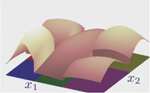
\includegraphics[width=0.5\textwidth, interpolate]{density-forest}
  \end{subfigure}
  \caption{Density Forest}
\end{figure}

\paragraph{Note} that the fitted densities have discontinuities at the splitting boundaries (this is the same type of discontinuity that we observed for regression forests or classification forests).

\paragraph{Sampling from this generative model}
\begin{enumerate}
    \item Draw uniformily a random tree index \(t \in \{1, T\}\) to select a single tree in the forest
    \item Descend the tree
        \begin{itemize}
            \item Starting at the root node, for each split node randomly generate the child index with probability proportional to the number of training points in edge (proportional to edge thickness)
            \item Repeat step 2 until a leaf is reached
        \end{itemize}
    \item At the leaf draw a random sample from the \textit{domain bounded} Gaussian stored at that leaf
\end{enumerate}

\begin{algorithm}[H]
\caption{Density Forest}
\begin{algorithmic}
  \REQUIRE Data matrix $\mat{X}\in\mathbb{R}^{n\times m}$, number of trees $\idx{n}{trees}$, number of thresholds $\idx{n}{thresh}$, tree depth $\idx{d}{tree}$
  %\STATE Initialize density matrix $\mat{D}\in\mathbb{R}^{n\times m}$
  \FOR {each tree}
    \FOR {root and all internal tree nodes}
      \FOR {all dimensions $1\dots m$}
        \FOR {$\idx{n}{thresh}$ random thresholds between the minimum and maximum of that dimension}
          \STATE Split data at threshold and compute information gain 
            \begin{equation*}
              I = H(S_j) - \sum_{\mathclap{i \in \{L,R\}}}\ \ \frac{|S^i_j|}{|S_j|} H\left(S^i_j\right)
            \end{equation*}
        \ENDFOR
        \STATE Split data at threshold which produced the highest information gain
        \STATE Save the index, which each feature vector had in $\mat{X}$
      \ENDFOR
    \ENDFOR
    \STATE Initialize distribution matrix of current tree $\mat{G}^{(t)}\in\mathbb{R}^{n\times m}$
    \FOR {all leafs}
      %\STATE Compute the marginal distribution
      \STATE Fit a Gaussian distribution to the leaf data
    \ENDFOR
  \ENDFOR
  \ENSURE The average of the distributions of all trees $\mat{D}=\frac{1}{\idx{n}{trees}}\sum_t\mat{G}^{(t)}$
\end{algorithmic}
\end{algorithm}


\subsection{Manifold Forest (Manifold Learning with Random Forests)}
\paragraph{Idea:} Learn a partitioning of the feature space by training a \underline{density forest.}\footnote{Note that we don't explicitly use the density} These partitions define a local neighborhood of the samples, which can be used to compute \underline{affinities}\footnote{Affinity intuition: Decreases with increasing distance}, and then to apply \eg \underline{Laplacian Eigenmaps} on them.

\paragraph{Task} Define affinities on a readily trained density forest.

Let \(w_{ij} = \euler^{-Q(\vec{x}_i, \vec{x}_j)}\) denote the affinity between samples \(\vec{x}_i, \vec{x}_j\), where \(Q(\vec{x}_i, \vec{x}_j)\) denotes a distance function.

The ``specialty'' of a Manifold Forest (in contrast, \eg to standard Laplacian Eigenmaps) is that these distances are defined \wrt the leafs of the trees (\ie the partitions).

\bigbreak

Example choices of \(Q\): Let \(\vec{d}_{ij} = \vec{x}_i - \vec{x}_j\), then

\begin{align*}
  \text{Mahalanobis: } Q(\vec{x}_i, \vec{x}_j) &= \begin{cases} \vec{d}_{ij}^T\left(\mat{\Lambda}_{l(\vec{x}_i)}\right)^{-1}\vec{d}_{ij} & \text{if in the same leaf } l(\vec{x}_i) \\ \hfil \infty & \text{otherwise} \end{cases} \\
  \text{Binary: } Q(\vec{x}_i, \vec{x}_j) &= \begin{cases} \hfil 0 & \text{if in the same leaf} \\ \infty & \text{otherwise} \end{cases}
\end{align*}

\[\text{Gaussian:} ...\]

In a single tree, only the samples within the same leaf-node have a non-zero affinity. Thus, a single tree produces a number of disconnected neighborhoods.
However if the affinities are averaged over the whole forest, all points become connected.

\begin{itemize}
  \item[\(\Rightarrow\)] We have a full adjacency matrix \(\mat{A} = \frac{1}{T} \sum_{t=1}^T w_{ij}^t\), where \(T\) denotes the total number of trees.
  \item[\(\Rightarrow\)] Compute LE on \(\mat{A}\).
\end{itemize}

\paragraph{Note} that the graph Laplacian in Criminisi/Shotton  are differently normalized, but it is the same algorithm:
\[\mat{L} = \mat{I} - \mat{\Gamma}^{-\frac{1}{2}} \mat{A} \mat{\Gamma}^{-\frac{1}{2}}\]
where \(\mat{\Gamma} = \mat{D} = \sum_{i,j} \mat{A}_{ij}\) denotes the sum of the weights for sample \(\vec{x}_i\).\footnote{just for normalization}

\bigbreak
\(\Rightarrow\) analogous to LE eigenvalue decomposition, arrange \(d'\) eigenvectors that are associated with the lowest eigenvalues in a matrix $\mat{E}$.

\[\mat{E} = (\vec{e}_1, \vec{e}_2, \dots, \vec{e}_d')\]

The projection of \(\vec{x}_i\) onto a \(d'\) dimensional space just corresponds to the \(i\)-th row of \(\mat{E}\). (note: drop the first eigenvector, where the eigenvalue is 0)

\paragraph{Advantages:}
\begin{enumerate}
  \item Automatic selection of discriminative features via information-based energy optimization
  \item Automatic estimation of the optimal dimensionality of the target space
  \item Being part of a more general forest model and, in turn code re-usability
\end{enumerate}
